\documentclass[tikz,border=10pt]{standalone}
\usepackage{mathrsfs}
\usepackage{physics}
\usetikzlibrary{decorations.pathmorphing}
    % this is for graphics. e.g. rectangle on title page
\usetikzlibrary{3d}
\usetikzlibrary{backgrounds}
\usetikzlibrary{arrows,shapes,positioning,shadows,trees,mindmap}
\usetikzlibrary{tikzmark}
\usetikzlibrary{calc,math}

\usepackage{tikz-3dplot}
\usepackage{pgfplots}
\pgfplotsset{compat = newest}
%\usepgfplotslibrary{colormaps}
\usepgflibrary{shapes.geometric}

\usepackage[edges]{forest}
\usetikzlibrary{arrows.meta}
\colorlet{linecol}{black!75}
\usepackage{xkcdcolors} % xkcd colors

\usetikzlibrary{patterns}
\tikzset{>={Stealth[inset=0pt,angle=20:10pt]}}


\tikzset{zigzag/.style={decorate,decoration=zigzag}}


\begin{document}
\tikzset{every picture/.style={line width=0.75pt}} %set default line width to 0.75pt        

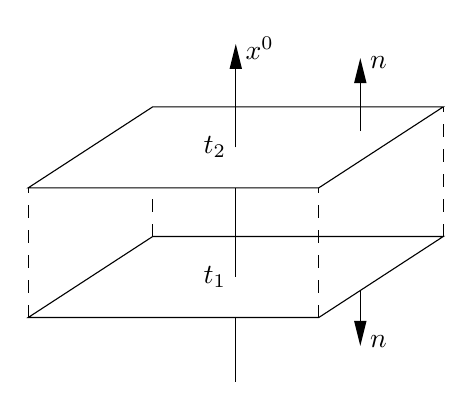
\begin{tikzpicture}[x=0.75pt,y=0.75pt,yscale=1,xscale=1]
%uncomment if require: \path (0,300); %set diagram left start at 0, and has height of 300

%Straight Lines [id:da7561920057223155] 
\draw    (168,60.63) -- (168,24.57) node[right]{$n$};
\draw [shift={(168,22.57)}, rotate = 90] [fill={rgb, 255:red, 0; green, 0; blue, 0 }  ][line width=0.08]  [draw opacity=0] (12,-3) -- (0,0) -- (12,3) -- cycle    ;
%Straight Lines [id:da9390201832362854] 
\draw    (108,55.75) -- (108,5) ;
%Shape: Parallelogram [id:dp3076157625737719] 
\draw  [fill={rgb, 255:red, 255; green, 255; blue, 255 }  ,fill opacity=1 ] (68,75.28) -- (208,75.28) -- (148,36.23) -- (8,36.23) -- cycle ;
%Straight Lines [id:da8578865318191331] 
\draw  [dash pattern={on 4.5pt off 4.5pt}]  (8,36.23) -- (8,98.7) ;
%Straight Lines [id:da7072572536191217] 
\draw  [dash pattern={on 4.5pt off 4.5pt}]  (68,75.28) -- (68,137.74) ;
%Straight Lines [id:da3301303971374956] 
\draw  [dash pattern={on 4.5pt off 4.5pt}]  (208,75.28) -- (208,137.74) ;
%Straight Lines [id:da8193356897666546] 
\draw  [dash pattern={on 4.5pt off 4.5pt}]  (148,36.23) -- (148,98.7) ;
%Straight Lines [id:da26369154168751474] 
\draw    (108,118.22) -- (108,55.75) node[left]{$t_1$};
%Shape: Parallelogram [id:dp8784333093732601] 
\draw  [fill={rgb, 255:red, 255; green, 255; blue, 255 }  ,fill opacity=1 ] (68,137.74) -- (208,137.74) -- (148,98.7) -- (8,98.7) -- cycle ;
%Straight Lines [id:da3281970419106002] 
\draw    (108,118.22)node[left]{$t_2$} -- (108,166) node[right]{$x^0$};
\draw [shift={(108,168)}, rotate = 270] [fill={rgb, 255:red, 0; green, 0; blue, 0 }  ][line width=0.08]  [draw opacity=0] (12,-3) -- (0,0) -- (12,3) -- cycle    ;
%Straight Lines [id:da020788736773178274] 
\draw    (168,126.03) -- (168,159.17) node[right]{$n$};
\draw [shift={(168,161.17)}, rotate = 270] [fill={rgb, 255:red, 0; green, 0; blue, 0 }  ][line width=0.08]  [draw opacity=0] (12,-3) -- (0,0) -- (12,3) -- cycle    ;
\end{tikzpicture}
\end{document}